\documentclass{report}
\usepackage[utf8]{inputenc}
\usepackage{array}
\usepackage{blindtext}
\usepackage{hyperref}
\usepackage{wrapfig}
\usepackage{multirow}
\usepackage{graphicx}
\usepackage{tabularx}
\usepackage{geometry}
\usepackage{changepage}
\usepackage{longtable}


\makeatletter
%same as \subsubsection but @level 4
\renewcommand\paragraph{\@startsection{paragraph}{4}{\z@}%
{-3.25ex\@plus -lex \@minus -.2ex}%
{1.5ex \@plus .2ex}%
{\normalfont\normalsize\bfseries}}

% number \paragraph
\setcounter{secnumdepth}{4}

\makeatother


\title{\normalsize {SOEN 6481 Summer 2021}\\[1.0cm]
\huge \textbf{\uppercase{Vision Document}} \\
\huge \textbf{\uppercase{e-concordia drive}}\\
\normalsize \vspace*{2\baselineskip}
}
\author{{Tavtej Singh Lehri\\
StudentID - 40121745}}
\date{August 17,2021}
%Title and Front page

\hypersetup{
    colorlinks=true,
    linkcolor=black,
    filecolor=magenta,      
    urlcolor=cyan,
    pdftitle={Delivery3 40121745},
    pdfpagemode=FullScreen,
    }
    
\urlstyle{same}

\begin{document}
\maketitle

\tableofcontents
\clearpage

\chapter{Vision Document}
\section{Introduction}
\subsection{Purpose}
The purpose of this vision document is to collect and analyze all assorted ideas that have come up to define the system, its requirements with respect to end users. Also, we shall predict and sort out how we hope this product will be used in order to gain a better understanding of the project, outline concepts that may be developed later, and document ideas that are being considered, but may be discarded as the product develops.[1]

\subsection{Scope}
E-Concordia drive is an E-learning platform for students to learn and practice driving lessons to obtain a license. It has got three main users: Trainer, Student and Admin.
Admin edits, comments, approves and publishes  lessons uploaded by a trainer.
Once approved the content is ready to be viewed by students.

\subsection{References}
{\footnotesize[1] R.Morales, 1b-p1 Vision Document, Available on:
https://moodle.concordia.ca/moodle/mod/resource/view.php?id= 2764233 [Current July, 2021]}\\

{\footnotesize[2]Improvement of Detection for Warning Students in E-learning Using Web Cameras - Scientific Figure on ResearchGate. Available from: https://www.researchgate.net/figure/A-block-diagram-of-the-e-learning-system\_fig1\_275541493 [accessed 13 Jul, 2021]}


\section{Positions}

\subsection{Problem Statement}

\begin{longtable}{|p{4.5cm}|p{11.5cm}|}
\hline
\textbf{The Problem of} & Not being able to hold in-person learning and practice for obtaining driver's license due to COVID-19 \\ \hline
\textbf{Affects} & All people who are new to driving and existing course students. \\ \hline
\textbf{The impact of which is} & That due to the pandemic the driving school had to close the in-person classes. \\ \hline
\textbf{The Solution to which is} & Creating an E-Learning website using which, the students can watch training videos prepared by instructors. Also based on the training module students can solve quizzes, which will help them practice for the main exam.\\ \hline
\caption{Problem Statement.\label{long}}
\end{longtable}


\subsection{Product Position Statement}

\begin{longtable}{|p{4.5cm}|p{11.5cm}|}
\hline
\textbf{For} & All people who are new to driving and existing course students\\ \hline
\textbf{Who}& Want to practice for the final driving exam.\\ \hline
\textbf{The E-Concordia Drive} & is an e-learning web product\\ \hline
\textbf{That} & helps students prepare for their final writing test, while sitting at their home.\\ \hline
\textbf{Unlike} & attending school amidst of the pandemic \\ \hline
\textbf{Our Product} & Helps the student learn from the vicinity of their homes. Using this platform they have access to videos 24/7, which helps revisit the videos them with if they did not understand something at first. Apart from this the platform also helps with practice quizzes.\\ \hline
\caption{Position Statement.\label{long}}
\end{longtable}

\section{Stakeholder Description}

\subsection{Stakeholder Summary}


\begin{longtable}{|p{4.5cm}|p{4.5cm}|p{6.5cm}|}
\hline
\textbf{Name} & \textbf{Description} & \textbf{Responsibilities} \\ \hline
Owner of Driving School & Person who owns the school and wants to take things online.&Should provide feedback and connect with Product Owner to convey his needs to the development team\\ \hline
Product Owner & A person who tells his needs to the business analyst & Should coordinate with BA to communicate the needs of business from the website.\\ \hline
Business Analyst & Is a person responsible for the SRS document and understanding the business needs & Should prepare SRS document and any changes to it, understand the business requirements, understand the customer requirements, layout clear and precise requirements for the developers and testers.\\ \hline
Architects & Acts as development lead and is a guy who has knowledge of MVC architecture  & Create the MVC style architecture for the developers, communicate with business and clients to design and execute solutions. Make executive software design decisions\\ \hline
Developers & Coders of the website & They are responsible to write a stable, understandable and easily executable PHP language based website. Should be familiar with MVC architecture. Should be able to read and understand requirements from the requirement document\\ \hline
Database Admins & Is a person who maintains and develops database for the application. & Should be familiar with MySQL database. Responsible for creating and maintaining the database. Should have in-depth knowledge of SQL.\\ \hline
QA/Test Analyst & Is a person who can find bugs in the application and help achieve stable application & Should be familiar with JIRA, can create test suite, test plan, test cases.\\ \hline
Marketing \& Advertising & A firm responsible to bring the application to end users. & Select the target users, advertise to the users, maintain social media advertising and help in SEO. \\ \hline
\caption{Stakeholder Summary.\label{long}}
\end{longtable}


\subsection{User Summary}

\begin{longtable}{|p{3.5cm}|p{3.5cm}|p{4.5cm}|p{4cm}|}
\hline
\textbf{Name} & \textbf{Description} & \textbf{Responsibilities} & \textbf{Stakeholder}\\ \hline
Students & Is a person who is enrolled for the driving lesson & Should register for the lessons, attend all the lectures and attempt all the quizzes & Self-Represented \\ \hline
Trainer & Is a person who takes the lessons & Is responsible for creating all the content for the students to view & Self-Represented \\ \hline
Admin & Is a person who maintains the content and users  & Is responsible for approval of all the contents and approval of students and trainers & Self-Represented \\ \hline
Marketer \& Advertiser & Is a person who advertises the website & Obtains the information to be advertised from the website and admins & Self-Represented.\\ \hline
\caption{User Summary.\label{long}}
\end{longtable}

\clearpage
\subsection{User Environment}
\begin{itemize}
    \item\textbf{Tools used for the project:}
    \begin{itemize}
        \item \textbf{PhpStorm:} IDE for software development
        \item \textbf{JIRA:} To improve the management of new development and defects.
        \item \textbf{GitHub:} for configuration management of the source code, test code and data.
        \item \textbf{MySQL:} for creating and maintaining the data.
        \item \textbf{Overleaf:} for creating all project related documentations
    \end{itemize}
    \item\textbf{Team Structure:}
    \begin{itemize}
        \item There will be 1 software architect who will also act as the development manager. The development team will consist of 4-5 developers and will be lead by the architect. Number of developers will go down to 2 once the project is live.
        \item The testing team will have 4 testers. The 4 people includes a test lead and 3 test analysts. Number of testers will reduce to 1-2 once the project goes live.
        \item There will be 1 scrum master and 1 business analyst.
        \item 1 developer and 1 tester will be moved to maintenance team once the project is live and deal wil production issues. 
    \end{itemize}
    \item Development of the product will be done using agile methodologies. It will be divided in 3 iterations. Iteration 1 will be 8 weeks long, Iterations 2 and 3 each will be 4 weeks long.
    \item For this release the project will work on Google Chrome and Safari. Expansion of this project will see working on other web browsers available in the market. Also there is a plan to create an application after analyzing the response for the website.
    \item Users should have a browser enabled device for using the website. Also the devices they use should be capable of viewing video and audio clips.
    \item Marketers and Advertisers should be familiar with the SEO and SCO tools. They should track all the social media activities via twitter, facebook and instagram.
    \item Student users shall have access to all the videos and quizzes once they enroll for the course.
    \item Trainer users should be able to record, manage and publish the videos for the approval of admin. Also they should be able to create quizzes for students to practice.
    \item Admin shall have the access to approve/reject the published stuff by the trainers.
\end{itemize}

\subsection{Key Stakeholder or Users Needs}


\begin{longtable}{|p{2.5cm}|p{2.5cm}|p{3.5cm}|p{3.5cm}|p{3.5cm}|}
\hline
\textbf{Need} & \textbf{Priority} & \textbf{Concerns} & \textbf{Current Solution} & \textbf{Proposed Solution}\\ \hline

Login Page & High & Login page should be secure & None & Login page will use captcha and unique userIDs and password with specific criterion.\\ \hline
Receive notification when new video is uploaded & High & Volume of notifications & None & Users will be sent push notifications when changes are made or new content is available\\ \hline
Responsive Website & Medium & Website should respond to user's behavior and environment. & None & Use of HTML and CSS style coding for the front end. \\ \hline
Stable and Bug Free website & High & There will be defect leakage & None & Use the extensive testing technique, track the defects in JIRA, perform regression testing after each iteration. \\ \hline
Good quality for audio and video & High & A/V should work on all kinds on internet bandwidths& none & users will be provided an auto pixel setup which will adjust the quality depending on internet quality. \\ \hline
Data to be stored & High & All data on the website to be stored in a database & using paper trails & a centralized database will be used to store all the information. \\ \hline
An account to do the quality check of content & Medium & Admin has knowledge of content & None & Train the admin to use website and ask him to complete advanced driving training.\\ \hline
Marketing data & High & Marketers and advertisers should have access to the content & none & Marketers and Advertisers should coordinate with the admin to collect the necessary data. They should use SEO/SCO to promote the website in search engines.\\ \hline
\caption{Stakeholder and User needs.\label{long}}\\
\end{longtable}


\section{Product Overview}

\subsection{Product Perspectives}
This product will setup the servers using apache servers. The servers in the backend will have interactive session between the code and the database. All the data will be stored in the MySQL database. User will have the active web connection. Using that users will use the set URL parameters to access the website on their PC/mobile devices. Below is the block diagram for the e-learning website:
\begin{figure}[htb!]
    \centering
    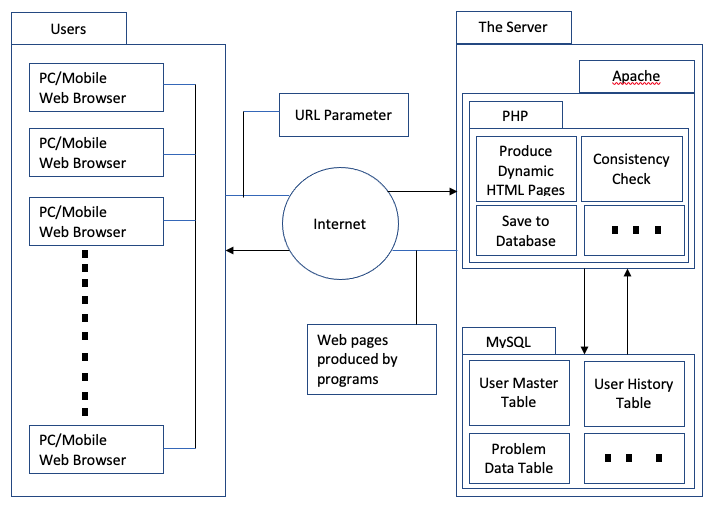
\includegraphics[scale=0.4]{1.png}
    \caption{A block diagram of the e-learning system [2] }
    \label{fig:my_label}
\end{figure}


\subsection{Assumptions and Dependencies}
\begin{longtable}{|p{5.5cm}|p{6.5cm}|}
\hline
\textbf{Assumptions} & \textbf{Dependencies} \\ \hline
It is assumed that there are enough resources to carry out the development of the project & In case of sick leaves or vacations a backup should be planned.\\ \hline
The server downtime should be planned for maintenance & Maintenance team is available and users are sent email for the downtime.\\ \hline
The website will work on latest versions Google Chrome and Safari & If any browser is discontinued then the document will change to introduce the new browser.\\ \hline
The developers have knowledge of PHP, HTML and CSS and MVC architecture & If not then the developers need to be trained which will add time to the project and scope will be revisited.\\ \hline
\caption{Assumptions and Dependencies.\label{long}}\\
\end{longtable}


\section{Product Features}
\textbf{Below listed are all the high level features of the website:}
\begin{enumerate}
    \item \textbf{Sign-Up:} All the end users should be able to create an account.
    \item \textbf{Login:} After the sign-up is complete, students will be given a studentID and traffic No, using this they can login. trainers and Admins can login with the username and password provided by the institute.\\[0.5ex]
    
    \clearpage
    \textbf{Students:}
    \item \textbf{Dashboard:}The dashboard page should have the general information about the type of license a student is training for.
    \item There will be 3 status of the modules: Completed,In Progress and Pending. Students cannot bypass the lessons and have to go sequentially.
    \item \textbf{Start Again} feature allows the student to preview the lesson contents again. Note: it will be available only after the lesson is complete.
    \item Lesson icons will have the slides count and the duration from the lesson content. This will help students track their individual lesson progress as well.
    \item Left pane on the dashboard page will have the Student ID and Examination ID along with next exam date, expiry dates of lesson and fees.
    \item Lessons will have an interactive screen. This will enable touchscreen device users no navigate easily. Videos will adjust to screen orientation of the mobile device.
    \item Description box will contain any extra information that the students nee to know.
    \item Volume adjustment button will be provided for the users to keep volume as per their need.
    \item Start, front and back button will help students navigate through slides
    \item Students when they logout will resume from where they left and will not have to start over again.
    \item Quiz related to the lesson will be enabled once a student completes their training video.
    \item Correct answer will be highlighted in green when students select the answer. If the student answer a wrong answer the answer will be marked in red and correct answer will be displayed in green.
    \item For match the following and rearranging the correct sequence, drag and drop feature will be provided.\\[0.5ex]
    
    \textbf{Trainers and Admins:}
    \item Dashboard page for the trainer login will have navigation pane with following links: Home, All Lessons, Pending, Drafts, Published, Notification. Navigation pane will be on all the pages in trainer account.
    \item Quick navigation will show the categorized number of all lessons, drafts, pending, notifications
    \item All lessons link will take the trainers to all lessons page where they will have manage lessons button.
    \item Manage lessons button will open a popover form where trainer will input the Lesson name(drop down menu as per SRS from EDC server), description, language (language listing as per SRS from EDC server) and icon to upload(using choose file button).
    \item Submit button in the popover form enables trainer to insert the content to lesson.
    \item A new pane is created in all lessons page for the lesson created with 5 buttons namely, Slide, Quiz,Lesson Status, Edit and Delete.
    \item Slide button is used for slide creation, Quiz button for quiz creation, lesson status shows the status of lesson in creation(Draft, Pending and Published). Edit and Delete.
    \item Plus button is used to expand the lesson and see the contents of it and lesson information pane on the right.
    \item when clicked on slide button the website will open an slide editor popover form.
    \item Media type in slide form will be audio, video and image. Slide duration is auto detected.
    \item Media file can be selected using the choose file button. Slide description is suitable for LTR or RTL.
    \item Slides are added after the user clicks on submit. The entry will have an icon for the notification on changes done by admin.
    \item Addition of Quiz also opens a popover pane. Quiz type will enable to select the type of quiz from, true/false, Right Answer, Drag and Drop and Reorder.
    \item For True/False space will be provided for trainer to type the question and provide the correct answer using dropdown.
    \item For choose correct answer Area to type question is given or it can be based on media(A/V or Image). 4 Answers will be typed in and the correct answer radio button will be selected by trainer.
    \item For drag and drop Questions will be typed in and matching answer will be given. System will shuffle the answers once the student is attempting the quiz.
    \item When trainer click on draft link on the navigation pane system navigates to the draft lessons page, where all the drafts are listed.
    \item When trainer click on published link on the navigation pane system navigates to the published lessons page, where all the published are listed.
    \item When the trainer click on notification, they will be navigated to the notifications page. It will display all the updates done either by trainer or admin.
    \item There will be 3 status of the updates: lesson updated(lesson creation, pending, draft and published), comment updated(when trainer updates admin comments), quality comment(from admin for trained)
    \item View button against the comments will take trainer to the slides having admin comments on it. Status of comment will change to done once changes are made and admin will be notified.
    \item Trainers will be allowed to create versions of the lessons they created using the edit button in the lesson management.
    \item No other trainer can work on the in progress work of a trainer. Only time when someone else can work on a trainer's pending work is when they are out of office or sick.
    \item Once the lesson is published trainer will loose access to edit or delete the slide and admin will have control over it.
    \item Admin has access to accept/reject students and trainers in case of change in their status
    
\end{enumerate}

\section{Other Product Requirements}
\begin{enumerate}
    \item Performance and Load testing to be done considering 350000 users at a time.
    \item A one time website navigation help to be provided for the users visiting for the first time.
    \item A help section to be provided which will have the website details for the users and ContactUS details.
    \item Product should comply with the existing HTML, TCP/IP and other web standards. 
\end{enumerate}

\section{Appendix}
\begin{table}[htb!]
    \centering
    \begin{tabular}{|p{5.5cm}|p{6.5cm}|}\hline
    \textbf{Section} & \textbf{Time Spent} \\ \hline
    Introduction & 1 hours \\ \hline
    Positions & 3 hours \\ \hline
    Stakeholder Descriptions & 8 hours \\ \hline
    Product Overview & 6 hours \\ \hline
    Product Features & 7 hours \\ \hline
    Other Product Requirements & 1 hour \\ \hline
    \textbf{Total} & \textbf{26 hours} \\ \hline
\end{tabular}
    \caption{Appendix - Vision Document}
    \label{tab:my_label}
\end{table}

\chapter{Defects and Inconsistencies Form}
\section{Task 1 - Identifying and finding inconsistencies in vision document}
\subsection{Defect Inspection Form}
\begin{longtable}{|p{0.5cm}|p{1.5cm}|p{2.5cm}|p{2.5cm}|p{4.5cm}|p{1.5cm}|p{1.5cm}|}
\hline
\textbf{ID}&\textbf{Location}&\textbf{Defect Type}&\textbf{Classification}&\textbf{Description}&\textbf{Status}&\textbf{Date Corrected}\\ \hline
1&2.1&Inadequacy&Minor&Impact has been mentioned as COVID-19 which has already been given in the problem&Closed&Aug 16\\ \hline
2&3.1&Omission&Major&Major Stakeholder is missing from the document. There is no owner of the driving school mentioned.&Closed&Aug 16\\ \hline
3&Sub-Sec 5 point 7&Inadequacy&Minor&Page is not mentioned on which the left pane will display the information&Closed&Aug 16\\ \hline
4&Sub-Sec 5 point 11&Over-specification&Minor&This requirement is mentioned for the developers to make them understand the functions needed.&Closed&Aug 16\\ \hline
5&Sub-Sec 5 point 40&Forward Reference&Minor&This requirement is mentioned keeping in mind that a trainer can also leave the institute and their credential will be revoked.&Closed&Aug 16\\ \hline
6&Sub-Sec 5 point 38&Contradiction&Major&When one trainer is busy no other trainer or admin is given access to modify that lesson.&Closed&Aug 17\\\hline
\caption{Defect Inspection Table.\label{long}}\\
\end{longtable}

\subsection{Inconsistencies Inspection Form}
\begin{longtable}{|p{0.5cm}|p{1.5cm}|p{2.5cm}|p{2.5cm}|p{4.5cm}|p{1.5cm}|p{1.5cm}|}
\hline
\textbf{ID}&\textbf{Location}&\textbf{Inconsistency Type}&\textbf{Classification}&\textbf{Description}&\textbf{Status}&\textbf{Date Corrected}\\ \hline
1&5 and 2.2&Terminology Clash&Weak&Term trainer, trainer and instructor is used to depict a person who creates training videos&Closed&Aug 17\\ \hline
2&5&Designation Clash&Weak&Term end users for E-Concordia User and Website User&Closed&Aug 17\\ \hline
3&Sub-Sec 5 point 18&Terminology Clash&Strong&In this section user means trainer or Admin where as in other places in the document user means Students as well.&Closed&Aug 17\\ \hline
\caption{Inconsistencies Inspection Table.\label{long}}\\
\end{longtable}

\section{Task 2 - Documenting Conflicts}
Based on the defects and inconsistencies below is the Interaction matrix for conflicts and overlapping\\[0.3cm]
\textbf{S1:}Students should be able to register on the portal.\\
\textbf{S2:}Trainer should record and upload course related videos.\\
\textbf{S3:}Admin should approve all the content uploaded by trainer.\\
\textbf{S4:}Students should be able to give Quiz after the lesson\\
\textbf{S5:}Students should be able to view the lessons and slides.
\begin{longtable}{|p{2cm}|p{1.5cm}|p{1.5cm}|p{1.5cm}|p{1.5cm}|p{1.5cm}|p{1.5cm}|}
\hline
\textbf{Statement}&\textbf{S1}&\textbf{S2}&\textbf{S3}&\textbf{S4}&\textbf{S5}&\textbf{Total}\\ \hline
\textbf{S1}&0&0&0&1000&1000&2000\\ \hline
\textbf{S2}&0&0&1000&1&1000&2001\\ \hline
\textbf{S3}&0&1000&0&1&1&1002\\ \hline
\textbf{S4}&1000&1&1&0&0&1002\\ \hline
\textbf{S5}&1000&1000&1&0&0&1002\\ \hline
\textbf{Total}&2000&2001&1002&1002&2002&7007\\ \hline
\caption{Interaction Matrix.\label{long}}\\
\end{longtable}


\section{Task 3 - Conflict Resolution}
\begin{enumerate}
    \item Consider the statement where admin is approving the content uploaded by the trainer.\\[0.3cm]
    \begin{table}[htb!]
        \centering
    \begin{tabular}{|p{3.5cm}|p{8.5cm}|} \hline
        \textbf{Avoiding Boundary Condition} & The conflict arises if both the trainer and the admin have access to approve the content. This will be considered as the boundary condition and restriction of access as per profiles will help in avoiding this.  \\ \hline
        \textbf{Weakening Conflict Statements} & To weaken the conflict approval of content rights should be kept with admin only.\\ \hline
    \end{tabular}
    \caption{CR-1}
        \label{tab:my_label}
    \end{table}
    \item The statements where trainer records and uploads the videos and student views the content is also a conflict.\\[0.3cm]
    \begin{table}[htb!]
    \centering
    \begin{tabular}{|p{3.5cm}|p{8.5cm}|} \hline
        \textbf{Avoiding Boundary Condition} & Allowing trainers to approve the content of the quiz avoid the boundary condition as he/she has more knowledge about the content of quiz and this way students can get quizzes sooner than expected.  \\ \hline
        \textbf{Weakening Conflict Statements} & Content will be viewed by students only when it is approved by admin not when a professor uploads it on the portal.\\ \hline
    \end{tabular}
    \caption{CR-2}
        \label{tab:my_label}
    \end{table}
\end{enumerate}

\section{Task 4 - Conflict Evaluation}
\begin{table}[htb]
    \centering
    \begin{tabular}{|p{3cm}|p{3cm}|p{3cm}|p{3cm}|}
\hline
\textbf{Evaluation Criteria NFR}&\textbf{Significance Weighting}&\textbf{Approval of Content}&\textbf{Viewing of Content}\\ \hline
\textbf{Fast Approval}&0.4&0.9&0.6\\ \hline
\textbf{Minimal Inconvenience}&0.2&0.6&1.0\\ \hline
\textbf{Right Content}&0.4&1.0&1.0\\ \hline
\textbf{Total}&1.0&0.88&0.64\\ \hline
\end{tabular}
    \caption{Conflict evaluation}
    \label{tab:my_label}
\end{table}

\section{Task 5 - Risk Management}
\subsection{Component Inspection}
    \begin{enumerate}
        \item \textbf{Student Module:} User should be above 16 years to obtain learner driver's permit and above 18 years to obtain full driver's permit. Student's video progress is not saved and they have to start videos again from the start. Student's response to quiz is not saved.
        \item \textbf{Trainer Module:}Trainer should have the license to teach, which is issued by government. Trainer's comments on the content is not posted or are not viewed by the admin.
        \item \textbf{Admin Module:}Risk will be that admin is not a certified quality assurance, so the content approved might be wrong. Trainer gets ambiguous comments from admin.
    \end{enumerate}

\subsection{Risk Tree}
    \begin{figure}[htb!]
    \centering
    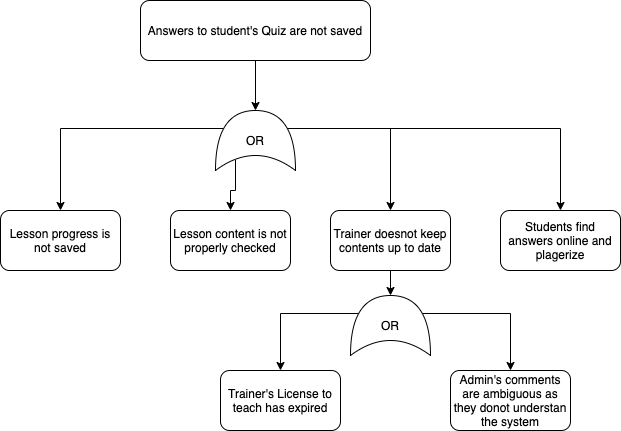
\includegraphics[scale=0.6]{D2.png}
    \caption{Risk Tree}
    \label{fig:my_label}
    \end{figure}

\clearpage    
\subsection{Risk Checklist}
    \begin{enumerate}
        \item Quantitative Risk Assessment \\
        \begin{longtable}{|p{4.5cm}|p{2.5cm}|p{4.5cm}|p{2.5cm}|} \hline
        Risk&Likelyhood(1-10)&Rationale&Severity(1-10)\\ \hline
        Answers to quiz not saved&5&This can happen due to loss of internet connection or a bug in the app, which questions stability.&5\\ \hline
        Admin's conmmets are ambiguous&6&Admin is not a trained professional in giving driving license so they might not be able to convey what is wrong with content.&8\\ \hline
        Loading video takes long time&8&Video content is not parsed properly which will question the system being less interactive and there might be lost of interest from students.&7\\ \hline
        Loss of life, students, trainers or admin&10&If admin's life is lost there will be no one to handover charge to new admin, it will take extra amount of money to find new trainer in case a trainer is lost.&10\\ \hline
        Data Leakage&7&Student's personal data is lost which questions database security.&10\\ \hline
        Database is not connected&4&Student data is not saved or content is not viewed to the students&10\\ \hline
        \caption{Risk Checklist.\label{long}}\\
        \end{longtable}
        
        \item Risk Control \\
        \begin{longtable}{|p{3.5cm}|p{3.5cm}|p{3.5cm}|p{3.5cm}|} \hline
        Risk&Countermeasure 1&Countermeasure 2&Evaluation of Countermeasure)\\ \hline
        Answers to quiz not saved&Student save each answer before moving to next one&System automatically saves answer when student moves to next question.&Option 2 is better as it reduces effort of student.\\ \hline
        Admin's comments are ambiguous&Admin should clearly mention what are the changes required&Trainer should ask admin what he meant by the comments before making changes.&Option 1 is more effective as option 2 increases time and cost.\\ \hline
        Loading video takes long time&Cloud based server should be used&Videos should be run on low quality.&option 1 is better as videos can be of any size and students should get best quality videos.\\ \hline
        Loss of life, students, trainers or admin&All trainers should know what others ar working on&Admin should also know how to add content.&both are equally viable option.\\ \hline
        Data Leakage&Use a layered architecture&Add security countermeasures and hire a 3rd party firm to handle the security.&Countermeasure 2 is better as school can hire a company which is expert is security.\\ \hline
        Database is not connected&Manually reconnect the database&If database is down for maintenance,keep database maintenance during the website maintenance time&both can equally be used depending on situation\\ \hline
        \caption{Risk Control.\label{long}}\\
        \end{longtable}
    \end{enumerate}
    

\section{Appendix}
\begin{table}[htb!]
    \centering
    \begin{tabular}{|p{5.5cm}|p{6.5cm}|}
\hline
\textbf{Section} & \textbf{Time Spent} \\ \hline
Task 1 & 2 hours \\ \hline
Task 2 & 1.5 hours \\ \hline
Task 3 & 3 hours \\ \hline
Task 4 & 1 hours \\ \hline
Task 5 & 1 hours \\ \hline
\textbf{Total} & \textbf{8.5 hours} \\ \hline
\end{tabular}
    \caption{Caption}
    \label{tab:my_label}
\end{table}

\chapter{Rebuttal Document: Response to reviewers, teacher assistant and instructor.}
\section{Introduction}
I would like to thank the reviewers, teacher assistant for their detailed feedback and useful suggestions to improve my vision document.\\[0.3cm]
I have carefully considered all the issues raised by my peers. Teacher assistant,  and instructor and prepared a revised vision document. This document outlines how I have addressed each comment individually. Each comment has been assigned a number R(1-3).C(1-N), where the number to the right of the R identifies the reviewer, and the number to the right of the C identifies the comment.\\[0.3cm]
My response to each comment is highlighted in blue.\\[0.3cm]
Sincerely,\\
Tavtej Singh Lehri

\section{Reviewer and Identifiers}
\begin{longtable}{|p{5.5cm}|p{6.5cm}|} \hline
\textbf{Reviewer}&\textbf{ID}\\ \hline
Peer 1(Comments Received in D2)& R1 \\ \hline
Peer 2(Comments Received in D2)& R2 \\ \hline
Teaching Assistant(Comments Received in D1)& R3\\ \hline
\caption{Reviewer and IDs.\label{long}}\\
\end{longtable}

\section{Reviewer Comments}
\color{blue}
\begin{enumerate}
    \item \textbf{R1.01:}Defect type changed from ambiguity to inadequacy.
    \item \textbf{R1.02:}Defect added as per comments
    \item \textbf{R1.03:}Changes made to interaction matrix.
    \item \textbf{R1.04:}NFRs are not changed as they are correct per my understanding. There is understanding clash between me and reviewer.
    \item \textbf{R1.05:}Risk Control added.
    \item \textbf{R2.01:}Overlaps Corrected.
    \item \textbf{R2.02:}Conflicts covered
    \item \textbf{R2.03:}Severity added in risk consequences table
    \item \textbf{R2.04:}Risk Control added.
    \item \textbf{R3.01:}Stakeholders Added.
    \item \textbf{R3.02:}Could not reduce pages even after change in formatting.
\end{enumerate}

\end{document}
